\documentclass[12pt]{report}
\usepackage[utf8]{inputenc}
\usepackage[russian]{babel}
%\usepackage[14pt]{extsizes}
\usepackage{listings}

% Для листинга кода:
\lstset{ %
language=go,                 % выбор языка для подсветки 
basicstyle=\small\sffamily, % размер и начертание шрифта для подсветки кода
numbers=left,               % где поставить нумерацию строк (слева\справа)
numberstyle=\tiny,           % размер шрифта для номеров строк
stepnumber=1,                   % размер шага между двумя номерами строк
numbersep=5pt,                % как далеко отстоят номера строк от подсвечиваемого кода
showspaces=false,            % показывать или нет пробелы специальными отступами
showstringspaces=false,      % показывать или нет пробелы в строках
showtabs=false,             % показывать или нет табуляцию в строках            
tabsize=2,                 % размер табуляции по умолчанию равен 2 пробелам
captionpos=t,              % позиция заголовка вверху [t] или внизу [b] 
breaklines=true,           % автоматически переносить строки (да\нет)
breakatwhitespace=false, % переносить строки только если есть пробел
escapeinside={\#*}{*)}   % если нужно добавить комментарии в коде
}

% Для измененных титулов глав:
\usepackage{titlesec, blindtext, color} % подключаем нужные пакеты
\definecolor{gray75}{gray}{0.75} % определяем цвет
\newcommand{\hsp}{\hspace{20pt}} % длина линии в 20pt
% titleformat определяет стиль
\titleformat{\chapter}[hang]{\Huge\bfseries}{\thechapter\hsp\textcolor{gray75}{|}\hsp}{0pt}{\Huge\bfseries}

%отступы по краям
\usepackage{geometry}
\geometry{verbose, a4paper,tmargin=2cm, bmargin=2cm, rmargin=1.5cm, lmargin = 3cm}
% межстрочный интервал
\usepackage{setspace}
\onehalfspacing
\usepackage{float}
% plot
\usepackage{pgfplots}
\usepackage{filecontents}
\usepackage{amsmath}
\usepackage{tikz,pgfplots}
\usetikzlibrary{datavisualization}
\usetikzlibrary{datavisualization.formats.functions}

\usepackage{graphicx}
\graphicspath{{src/}}
\DeclareGraphicsExtensions{.pdf,.png,.jpg}

\usepackage{geometry}
\geometry{verbose, a4paper,tmargin=2cm, bmargin=2cm, rmargin=1.5cm, lmargin = 3cm}
\usepackage{indentfirst}
\setlength{\parindent}{1.4cm}

\usepackage{titlesec}
\titlespacing{\chapter}{0pt}{12pt plus 4pt minus 2pt}{0pt}

\begin{filecontents}{timeAnts.dat}
	2 6.9806
	3 14.96
	4 22.9391
	5 35.9015
	6 52.8592
	7 71.8331
	8 93.7493
	9 117.7173
	10 147.609
\end{filecontents}
\begin{filecontents}{timeBrute.dat}
	2 0 
	3 0.9
	4 1
	5 1.4
	6 1.4
	7 2
	8 11.0021
	9 157.5722
	10 1523.9153
\end{filecontents}

\begin{document}
%\def\chaptername{} % убирает "Глава"
\begin{titlepage}
	\centering
	{\scshape\LARGE МГТУ им. Баумана \par}
	\vspace{3cm}
	{\scshape\Large Лабораторная работа №7\par}
	\vspace{0.5cm}	
	{\scshape\Large По курсу: "Анализ алгоритмов"\par}
	\vspace{1.5cm}
	{\huge\bfseries Поиск подстроки в строке\par}
	\vspace{2cm}
	\Large Работу выполнил: Мокеев Даниил, ИУ7-54\par
	\vspace{0.5cm}
	\Large Преподаватели:  Волкова Л.Л., Строганов Ю.В.\par

	\vfill
	\large \textit {Москва, 2019} \par
\end{titlepage}

\tableofcontents

\newpage
\chapter*{Введение}
\addcontentsline{toc}{chapter}{Введение}

Муравьиный алгоритм — один из эффективных полиномиальных алгоритмов для нахождения приближённых решений задачи коммивояжёра, а также решения аналогичных задач поиска маршрутов на графах.

Целью данной лабораторной работы является изучение муравьиных алгоритмов и приобретение навыков параметризации методов на примере муравьиного алгоритма, примененного к задаче коммивояжера.

Задачи данной лабораторной работы:
\begin{itemize}
	\item рассмотренть муравьиный алгоритм и алгоритм полного перебора в задаче коммивояжера;
	\item реализовать эти алгоритмы;
	\item сравнить время работы этих алгоритмов.
\end{itemize}


\chapter{Аналитическая часть}
В данной части будут рассмотрены существующие на данный момент алгоритмические решения проблемы поиска подстроки в строке. 

\section{Общие сведения об алгоритмах поиска подстроки}
\par
Поиск подстроки в строке — одна из простейших задач поиска информации. Сферы применения алгоритмов поиска включают в себя:
\begin{itemize}
	\item Текстовые редакторы;
	\item СУБД;
	\item компиляторы;
	\item программы определения проверки плагиата;
	\item поисковые системы;
	\item биоинформатика.
\end{itemize}
На сегодняшний день существует огромное разнообразие алгоритмов поиска подстроки. Программисту приходится выбирать подходящий в зависимости от таких факторов: длина строки, в которой происходит поиск, необходимость оптимизации, размер алфавита, возможность проиндексировать текст, требуется ли одновременный поиск нескольких строк.  В данной лабораторной работе будут рассмотремы два алгоритма сравнения с образцом, алгоритм Кнута-Морриса-Пратта и алгоритм Бойера-Мура.
\subsection{Стандартный алгоритм}
Стандартный алгоритм начинает со сравнения первого символа текста с первым символом подстроки. Если они совпадают, то происходит переход ко второму символу текста и подстроки. При совпадении сравниваются следующие символы. Так продолжается до тех пор, пока не окажется, что подстрока целиком совпала с отрезком текста, или пока не встретятся несовпадающие символы. В первом случае задача решена, во втором мы сдвигаем указатель текущего положения в тексте на один символ и заново начинаем сравнение с подстрокой\cite{2}.

\subsection{Алгоритм Бойера-Мура}
Алгоритм Бойера-Мура осуществляет сравнение с образцом справа налево, а не слева направо. Исследуя искомый образец, можно осуществлять более эффективные прыжки в тексте при обнаружении несовпадения. В этом алгоритме кроме таблицы суффиксов применяется таблица стоп-символов. Она заполняется для каждого сивола в алфавите. Для каждого встречающегося в подстроке символа таблица заполняется по принципу максимальной позиции символа в строке, за исключением последнего символа. При определении сдвига при очередном несовпадении строк, выбирается максимальное значение из таблицы суффиксов и стоп-символов\cite{2}.

\begin{center}
Таблица 2. Пошаговая работа алгоритма Бойера-Мура.\\
\begin{tabular}{| c | c | c | c | c | c | c | c | c | c | }
	\hline
	a&b&a&b&a&c&a&b&a&a \\
	\hline
	\hline
	a&b&a&\textcolor{red}{a}&&&&&&\\
	\hline
	&&a&b&a&\textcolor{red}{a}&&&&\\
	\hline
	&&&&&&\textcolor{green}{a}&b&a&a\\
	\hline
\end{tabular}
\end{center}


\subsection{Алгоритм Кнута-Морриса-Пратта}
Алгоритм Кнута-Морриса-Пратта основан на принципе конечного автомата, однако он использует более простой метод обработки неподходящих символов. В этом алгоритме состояния помечаются символами, совпадение с которыми должно в данный момент произойти. Из каждого состояния имеется два перехода: один соответствует успешному сравнению, другой - несовпадению. Успешное сравнение переводит нас в следующий узел автомата, а в случае несовпадения мы попадаем в предыдущий узел, отвечающий образцу. 
В программной реализации этого алгоритма применяется массив сдвигов, который создается для каждой подстроки, которая ищется в тексте. Для каждого символа из подстроки рассчитывается значение, равное максимальной длине совпадающего префикса и суффикса отсительно конкретного элемента подстроки. Создание этого массива позволяет при несовпадении строки сдвигать ее на расстояние, большее, чем 1 (в отличие от стандартного алгоритма).

\begin{center}
	Таблица 1. Пошаговая работа алгоритма Кнута-Морриса-Пратта.\\
	
	\begin{tabular}{| c | c | c | c | c | c | c | c | c | c | }
		\hline
		a&b&a&b&a&c&a&b&a&a \\
		\hline
		\hline
		a&b&a&\textcolor{red}{a}&&&&&&\\
		\hline
		&&a&b&a&\textcolor{red}{a}&&&&\\
		\hline
		&&&&a&\textcolor{red}{b}&a&a&&\\
		\hline
		&&&&&\textcolor{red}{a}&b&a&a&\\
		\hline
		&&&&&&a&b&a&\textcolor{green}{a}\\
		\hline
	\end{tabular}
\end{center}

\section*{Вывод}
\addcontentsline{toc}{section}{Введение}
В данном разделе были рассмотрены алгоритмы для решения задачи поиска подстроки в строке. 


\chapter{Конструкторская часть}
В данном разделе будут рассмотрены основные требования к программе и схемы алгоритмов.

\section{Требования к программе}
\textbf{Требования к вводу:}
\begin{itemize}
	\item Подаются не пустые подстрока и строка;
	\item длина подстроки меньше, чем длина строки.
\end{itemize}

\textbf{Требования к программе:}
\begin{itemize}
	\item Программа должна возвращать первое индекс первого вхождения подстроки.
\end{itemize}
.  
\newline  
\textbf{Входные данные} - на вход подается строка и подстрока;
\newline
\textbf{Выходные данные} - программа возвращает индекс первого вхождения подстроки в строку, если вхождения не было возвращается -1.

\section{Схемы алгоритмов}
В данном разделе будут приведены схемы алгоритмов для решения задачи поиска подстроки в строке:
Бойера-Мура(Рис.\ref{fig:BM}) и Кнута-Морриса-Пратта (Рис. \ref{fig:KMP})\\
\begin{figure}[!htbp]
	\centering
	\includegraphics[width=1.1\linewidth]{bm_matrix_easy_graphml.png}
	\caption{Схема алгоритма Бойера-Мура}
	\label{fig:BM}
\end{figure}
\begin{figure}[!htbp]
	\centering
	\includegraphics[width=1\linewidth]{kmp_graphml_graphml.png}
	\caption{Схема алгоритма Кнута-Морриса-Пратта}
	\label{fig:KMP}
\end{figure}


\section*{Вывод}
\addcontentsline{toc}{section}{Вывод}
В данном разделе были рассмотрены требования к программе и схемы алгоритмов.


\chapter{Технологическая часть}

\section{Выбор ЯП}
В качестве языка программирования был выбран golang.
Время работы алгоритмов было замерено с помощью time. 
\section{Описание структуры ПО}
В данном разделе будет рассмотрена структура ПО (Рис. \ref{fig:mpr})
\begin{figure}[!htbp]
	\centering
	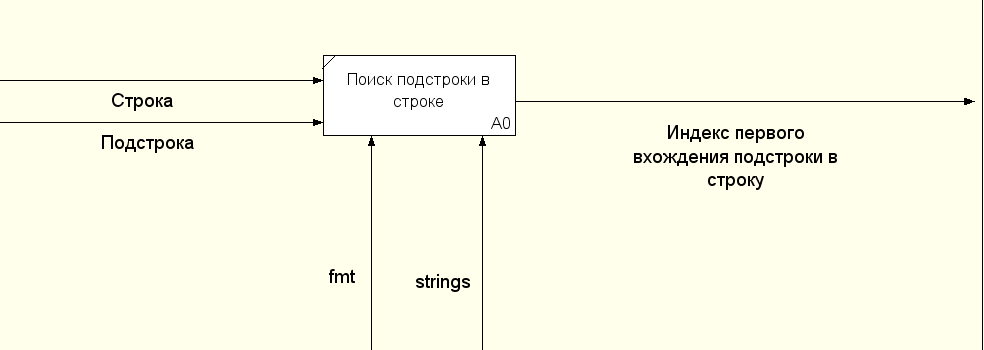
\includegraphics[width=1.1\linewidth]{lab07ram.png}
	\caption{Функциональная схема поиска подстроки в строке (IDEF0 диаграмма 1 уровня)}
	\label{fig:mpr}
\end{figure}
\section{Сведения о модулях программы}
Программа состоит из:
\begin{itemize}
	\item main.go- главный файл программы, в котором располагается точка входа в программу.
	\item estim.go - файл содержащий функции замера времени.
\end{itemize}
\section{Примеры работы}
В данном разделе приведен пример работы программы (Рис. \ref{ris:example})
\begin{figure}[h]
	\centering{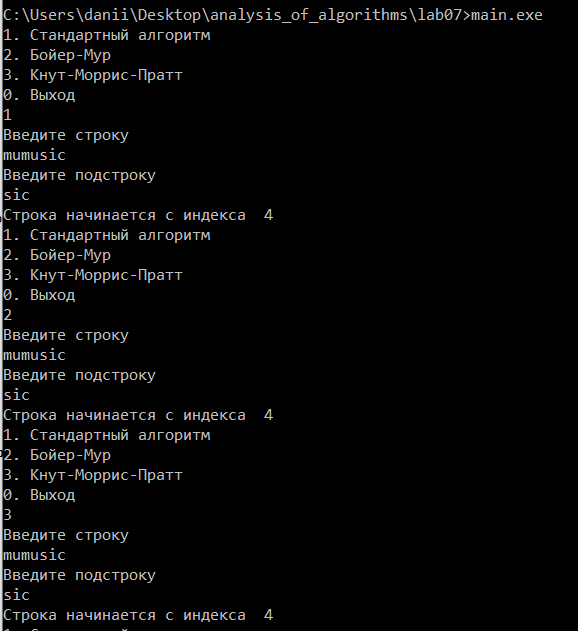
\includegraphics[scale=1.1]{example.png}} 
	\caption{Пример работы программы}
	\label{ris:example}
\end{figure}
\section{Листинг кода алгоритмов}
В данном разделе будут приведены листинги кода стандартного алгоритма поиска подстроки в строке (Листинг \ref{std}), алгоритма Бойера-Мура (Листинг \ref{BM}) и алгоритма Кнута-Морриса-Пратта (Листинг \ref{KMP})
\begin{lstlisting}[label=std,caption = Стандартный алгоритм поиска подстроки в строке, language = go]

func std(str, sub string) int{
	if len(sub) > len(str) || len(sub)== 0 || len(str) == 0{
		return -1
	}
	
	flag := true
	for i:=0;i<len(str);i++{
		flag = true
		if str[i] == sub[0]{
			for j:=0;j<len(sub);j++{
				if str[i+j] != sub[j]{
					flag = false
				}
				if flag{
					return i
				}
			}
		}
	}
	return -1
}
\end{lstlisting}

\begin{lstlisting}[label=BM,caption = Алгоритм Бойера-Мура, language = go]
func get_table(substring string) map[rune]int {
	length := utf8.RuneCountInString(substring)
	runes := []rune(substring)
	
	table := make(map[rune]int)
	
	for i := 0; i < length; i++ {
		j := runes[i]
		table[j] = length - i - 1
	}
	return table
}

func BM(str, sub string) int{
	if len(sub) > len(str) || len(sub)== 0 || len(str) == 0{
		return -1
	}
	table := get_table(sub)
	strrunes := []rune(str)
	subrunes := []rune(sub)
	str_l := utf8.RuneCountInString(str)
	sub_l := utf8.RuneCountInString(sub)
	i:=sub_l-1
	j,k:=i,i
	for (j>=0 && i<=str_l-1){
		j = sub_l-1
		k = i
		for(j>=0 && (table[strrunes[k]] == table[subrunes[j]])){
			k--
			j--
		}
		if _,ok := table[strrunes[i]]; !ok{
			i+= sub_l
		}else{
			i+=table[strrunes[i]]
		}
	}
	if k>= str_l - sub_l{
		return -1
	} else {
		return k+1
	}
}
\end{lstlisting}
\begin{lstlisting}[label=KMP,caption = Алгоритм Кнута-Морриса-Пратта, language = go]
func get_preph(str string) []int{
	res := make([]int, len(str))
	for i:= 1; i<len(str);i++{
		j := res[i-1]
		for (j>0 && str[i] != str[j]){
			j = res[j-1]
		}
		if (str[i] == str[j]){
			j++
		}
		res[i] = j
	}
	return res
}

func KMP(str, sub string) int{
	if len(sub) > len(str) || len(sub)== 0 || len(str) == 0{
		return -1
	}
	
	tmp := []string{sub, str}
	str = strings.Join(tmp, "@")
	pr := get_preph(str)
	len_sub := len(sub)
	for i:=len_sub+1; i<len(str);i++{
		if pr[i] == len_sub{
			return i-2*len_sub
		}
	}
	return -1
}
\end{lstlisting}
\section*{Вывод}
\addcontentsline{toc}{section}{Вывод}
В данном разделе были рассмотрены основные сведения о модулях программы и листинг кода алгоритмов.


\chapter*{Заключение}
\addcontentsline{toc}{chapter}{Заключение}
Были реализованы и изучены основные существующие алгоритмы поиска подстроки в строке - стандартный тривиальный алгоритм, алгоритм Бойера-Мура и алгоритм Кнута-Морриса-Пратта.


\addcontentsline{toc}{chapter}{Список литературы}
\begin{thebibliography}{3}
	\bibitem{1} Окулов С. М. Алгоритмы обработки строк. — М.: Бином, 2013. — 255 с.
	\bibitem{2} Дж. Макконнелл. Анализ лгоритмов. Активный обучающий подход
	\bibitem{UnitTests}
	Основные сведения о модульных тестах [Электронный ресурс], - режим доступа: https://docs.microsoft.com/ru-ru/visualstudio/test/unit-test-basics?view=vs-2019
\end{thebibliography}


\end{document}

